\documentclass[12pt]{article}    % <--- 12pt font
\usepackage{graphicx} % Required for inserting images
\usepackage[margin=1in]{geometry}% <--- 1 in margin
\usepackage{setspace}
\doublespace                      % <--- double space
% \usepackage{lipsum}
\usepackage{natbib}
\usepackage{amsmath}
\usepackage[
backend=biber,
style=ieee,
]{biblatex}
\addbibresource{refs.bib} 

\title{Scraping and Analyzing Movie Reviews}
\author{Shadi Hamdan, 61969}
\date{January 2024}

\begin{document}
\maketitle

\section{Introduction}

In today's digital age, the internet plays a vital role as a rich source of data, with many people using it for entertainment, such as watching movies and shows. Various websites have emerged to aggregate information about films and TV series, making it convenient for users to access details about their favorite media content. Among these, IMDB, or the internet movie database, stands out as the most popular platform. It not only provides comprehensive information about movies and TV shows but also serves as a central hub for sharing reviews and rating films. In the context of this project, the goal is to leverage this widely-used website to create a substantial dataset of movie reviews, surpassing 100,000 reviews, which is larger than any other publicly available IMDB dataset to the best of the author's knowledge. The primary objective is to then analyze these reviews to gain insights, with a specific focus on understanding the relationship between the content of the written textual reviews and the assigned review scores. The aim of this project is twofold. First, to share the dataset publicly as a potentially useful resource for other researchers. Secondly, the aim is to explore patterns and correlations within the vast realm of movie reviews available online.

\section{Dataset}

To analyze movie reviews and ratings, we need a dataset of textual reviews along with their ratings. However, existing datasets such as the Large Movie Review Dataset \cite{maas-EtAl:2011:ACL-HLT2011} only include a binary postive/negative rating instead of the full scale 1-10 star review system that IMDB uses. This limits the possible analyses to mostly binary classification tasks. We aim to have a dataset that does not have this limitation in order to enable researchers to be more flexible and open up avenues to different tasks and analyses.

As a result, we first scrape reviews directly from IMDB, and include the full review text and the corresponding score. 

\subsection{Scraping}

The format of IMDB is pretty straightforward. Each title, whether it is a movie or a specific TV show episode, is designated by a unique identifier, called \textit{tconst}. Given \textit{tconst}, the page for the title can be immediately accessed at the following URL using the same template: 

\begin{align*}
    \text{imdb.com/title/\textit{tconst}/}
\end{align*}

Moreover, each title also has a list of user submitted reviews. These reviews can be accessed at: 

\begin{align*}
    \text{imdb.com/title/\textit{tconst}/reviews}
\end{align*}

Within this review page, the reviewss are listed one after the other, each with its own text and assigned score. 

The format of \textit{tconst} is also pretty consistent. It always starts with \textit{tt} followed by 7 to 8 numbers. The titles are also assigned consecutively, with the earliest title starting at \textit{0000001}, and increasing as more titles are added. As a result, it is possible to iterate over all titles by iterating one by one. However, many titles are either very old or have no details. As a result, we looked for a better way to iterate over movies.

IMDB also has publicly available datasets for non-commercial usage. One such dataset, released with the name \textit{title.basics.tsv.gz}, contains all titles found on IMDB, with their unique alphanumeric ID \textit{tconst}. As a result, we choose to use this file as a starting point.

After accessing the title dataset, we randomly shuffle the dataset and start iterating over the titles one by one. We immediately access the review page and scrape available reviews. We limit the number of reviews to a maximum of 25 reviews per title. This is to avoid a few very popular titles from dominating the dataset, and as a result to have a more even distribution across titles.

To scrape the reviews, we use the requests python library in order to get the HTML of the review page. Then, we use the Scrapy library in order to extract the relevant information from the HTML page. To avoid getting rate limited by IMDB, we add a wait time of 1-5 seconds between every request.

In the end, over 250000 separate titles were accessed in order to scrape reviews. With an average of 3 second per request, this took over a week of scraping in order to do. More details about the resulting dataset can be found in the next section. 

\subsection{Resulting Data Statistics}

Out of the 250000 accessed titles, a large majority had no reviews, since a small minority of titles contained the most reviews. Out of the 250000, only 19705 titles had reviews. The majority of the reviews ended up having 5 or less reviews. The exact distribution of number of reviews per title can be seen in Figure \ref{fig:review_hist}.

\begin{figure}
    \centering
    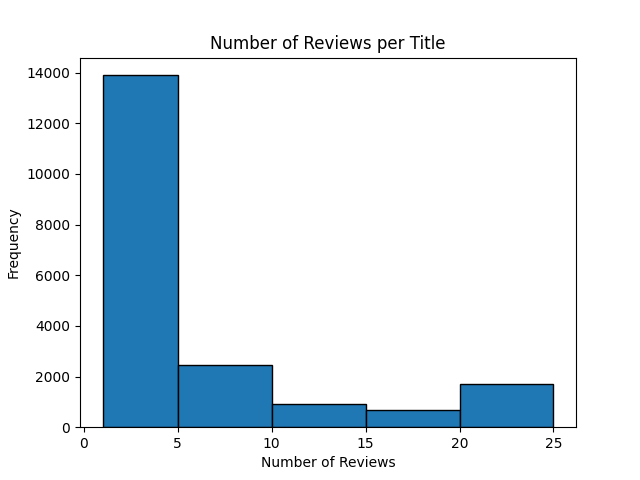
\includegraphics[width=0.7\linewidth]{reviews_histogram.png}
    \caption{Number of reviews a title has. The majority of titles have 1-5 reviews, with the next most common amount being 6-10 and 21-25 reviews.}
    \label{fig:review_hist}
\end{figure}

The histogram of reviews also shows the importance of limiting the number of reviews to 25. If not for the limit, the dataset would be dominated by these very popular titles with many reviews. This could easily result in a biased analysis, as there are many confounding factors in reviews. For example, the name of the main character in a very popular and critically acclaimed movie would be a very strong sign that the review rating is high, which is undesirable if what we want to analyse is the content of the review and not simply memorize which characters are in good movies and vice versa.

The length of most reviews tends to be under 4000 characters. However, there is a significant number of reviews that are longer than that. The histogram of review lengths can be found in Figure \ref{fig:len_hist}. This introduced a concern of review length for our analyses, which we will discuss more in the next section.

\begin{figure}
    \centering
    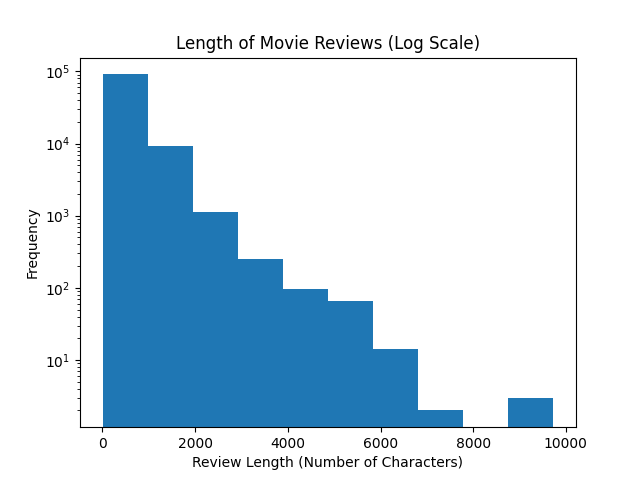
\includegraphics[width=0.7\linewidth]{length_histogram.png}
    \caption{Distribution of review lengths in characters. The majority of titles have under 4000 characters, but a significant portion of reviews are very long.}
    \label{fig:len_hist}
\end{figure}

\subsection{Data Preprocessing}

To improve the interpretability of the dataset, we first split the reviews into 4 semantic classes: 

\begin{itemize}
    \item Very Negative: This consists of reviews with a rating between 1 and 3, the lowest possible scores on IMDB.
    \item Negative: This consists of reviews with a rating of 4 and 5, which denotes somewhat negative reviews.
    \item Positive: This consists of reviews with a rating of 6 and 7, which denotes somewhat positive reviews.
    \item Very Positive: This consists of reviews with a rating between 8 and 10, the highest possible scores on IMDB, which denotes a very critically acclaiming review.
\end{itemize}

Based on the distribution of ratings, we can see that the majority of reviews are very positive, with the next most common being positive. This is somewhat expected, as people tend to only write reviews if they have a strong opinion about a title, and people tend to only watch things they think they will like, and as a result the majority of reviews are either very positive, positive, or very negative. The prevalence of very negative reviews could denote viewers who had high expectations for a title and were disappointed, or viewers who were expecting a different type of movie and were disappointed. The distribution of ratings can be seen in Figure \ref{fig:rating_hist}. The least common type of review is negative, which could be due to the fact that people who dislike a title are less likely to write a review, or that people who really dislike a title are more likely to give it a very negative rating instead of a negative rating.

\begin{figure}
    \centering
    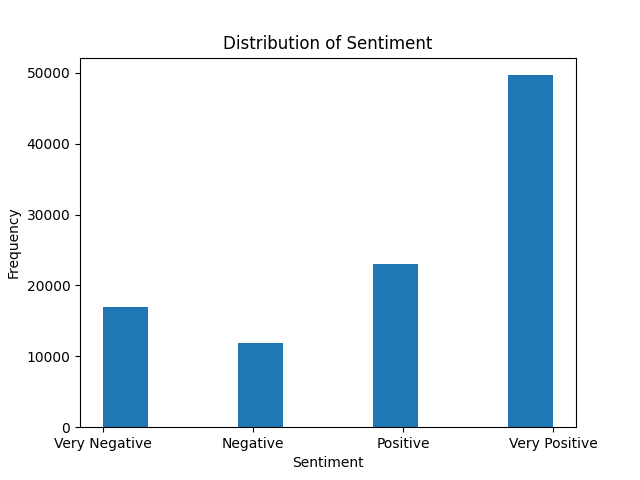
\includegraphics[width=0.7\linewidth]{sentiment_histogram.png}
    \caption{Distribution of sentiments in the dataset. As expected based on the rating distribution, most of the reviews are very positive.}
    \label{fig:sentiment_hist}
\end{figure}

% - Furthermore, I cleaned the text data using the Natural Language ToolKit, NLTK. I did three things: 
% -- Used stemming. Describe what stemming is in natural language processing and why it is used.
% -- Tokenization. Describe it similarly to stemming
% -- Lowercasing. Describe why it is important.

After splitting the reviews into semantic classes, we then cleaned the text data using the Natural Language ToolKit, NLTK. We used stemming, lemmatization, tokenization, and lowercasing. 

Stemming is the process of reducing words to their root form. For example, the words "running", "runs", and "ran" would all be reduced to "run". This is important because it reduces the number of unique words in the dataset, and as a result reduces the number of features in the dataset and combines words that have the same meaning. For example, "running" and "runs" would be combined into the same feature, which is important because they have the same meaning. Following the recommendation in the documentation, we used the SnowballStemmer, which is a stemming algorithm developed by Martin Porter.

Lemmatization is similar to stemming, but instead of reducing words to their root form, it reduces words to their lemma, which is the canonical form of a word. For example, "better" and "best" would both be reduced to "good". This is important because it reduces the number of unique words in the dataset, and as a result reduces the number of features in the dataset and combines words that have the same meaning. For example, "better" and "best" would be combined into the same feature, which is important because they have the same meaning. Following the recommendation in the documentation, we used the WordNetLemmatizer, which is a lemmatization algorithm developed by Princeton University.


Tokenization is the process of splitting a sentence into individual words. This is important because it allows us to count the number of times each word appears in a review, which is important for our analyses. We will discuss this more in the next section.

Finally, similarly to stemming, lowercasing is important because it reduces the number of unique words in the dataset. For example, "Running" and "running" would be combined into the same feature, which is important because they have the exact same meaning. Furthermore, we also remove all punctuation, as it is not important for our analyses.

\section{Experiments}

To start off, we have two main research questions that we aim to answer with our analyses:

\begin{itemize}
    \item Do the words used in a review have a good correlation with the assigned review score?
    \item Is it possible to predict the assigned review score based on the words used in the review?
\end{itemize}

To do so, we design two main experiments. In the first one, we try to cluster the reviews without access to their semantic classes based on the words used in the review, and then analyse these clusters. In the second one, we try to predict the assigned review score based on the words used in the review in order to see if there is a strong correlation between the words used and the assigned review score.

\subsection{Clustering}

In order to cluster the reviews, we first need to represent them in a way that is suitable for clustering. To do so, we use the bag of words model. The bag of words model is a simple representation of text that only counts the number of times each word appears in a document. This results in a vector of word counts for each document, which can then be used for clustering or other analyses.

However, the bag of words model has a few limitations. First, it does not take into account the order of words in a document. Secondly, it does not take into account the importance of words. For example, the word "the" would have the same representation as the word "movie", even though the word "the" is much more common and less important than the word "movie". 

An alternative representation of text is the TF-IDF representation. TF-IDF stands for term frequency-inverse document frequency. It is a representation of text that takes into account the importance of words. It is calculated by multiplying the term frequency, which is the number of times a word appears in a document which is a single review in our case, by the inverse document frequency, which is the number of reviews that contain the word. This results in a vector of TF-IDF scores for each review, which can then be used instead of the bag of words model for clustering or other analyses.


To cluster the reviews, we use the K-Means clustering algorithm. K-Means is a simple clustering algorithm that works by randomly initializing K centroids or clusters, and then iteratively updates the centroids and assigns each data point to the closest centroid. The number of clusters K is a hyperparameter that needs to be chosen. However, in our case, we know that there are 4 semantic classes, so we choose K=4. Then, we try to cluster the reviews using both the bag of words model and the TF-IDF model, and compare the results.


\begin{figure}[!ht]
    \centering
    \begin{subfigure}{0.8\textwidth}
        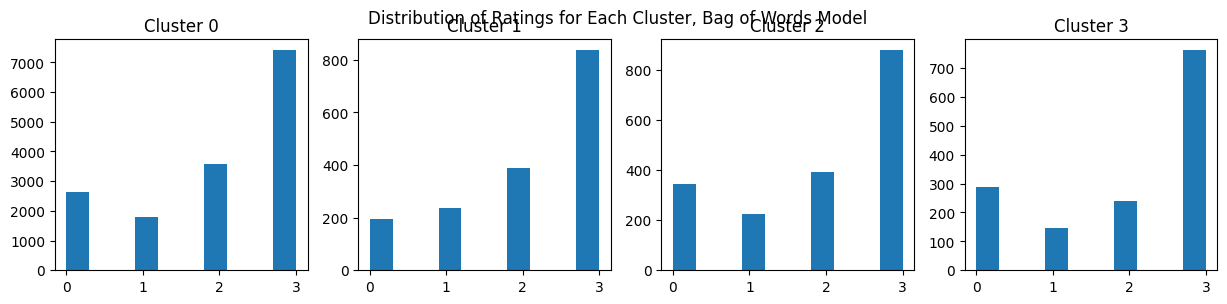
\includegraphics[width=\linewidth]{clusters_bow.png}
        \caption{Clusters of reviews using the bag of words model.}
        \label{fig:clusters_bow}
    \end{subfigure}
    \hfill
    \begin{subfigure}{0.8\textwidth}
        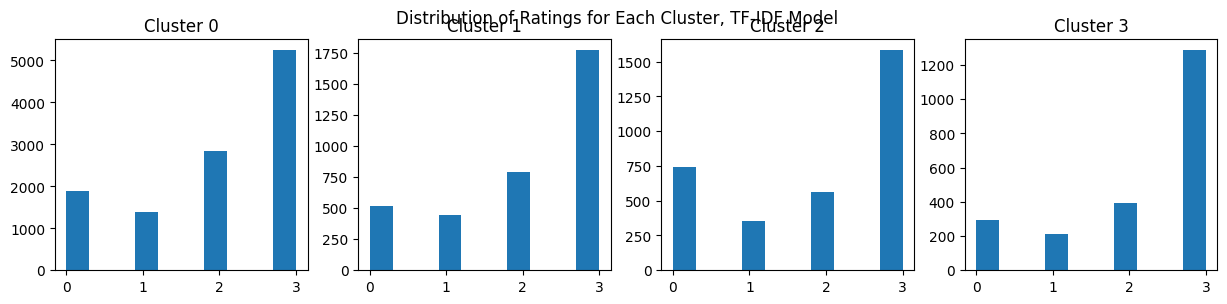
\includegraphics[width=\linewidth]{clusters_tfidf.png}
        \caption{Clusters of reviews using the TF-IDF model.}
        \label{fig:clusters_tfidf}
    \end{subfigure}
    \caption{Comparison of k-means clusters using the bag of words model and the TF-IDF model.}
    \label{fig:combined_clusters}
\end{figure}

The distribution of semantic classes within each of the clusters can be seen in Figure \ref{fig:combined_clusters}. As we can see, the clusters are very similar to the original distribution of the semantic classes, and the clustering fails to separate the reviews into any meaningful clustering in terms of semantics. This is the same whether we use the bag of words model or the TF-IDF model. This shows that using the words used in a review directly might result in features that are not easy to cluster. 

\begin{figure}
    \centering
    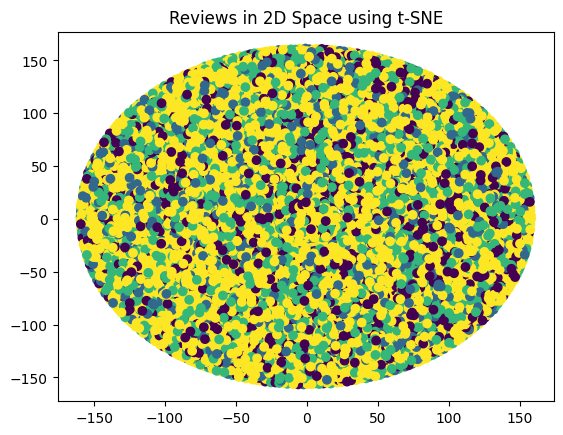
\includegraphics[width=0.7\linewidth]{tsne_clusters.png}
    \caption{Clusters of reviews using t-SNE.}
    \label{fig:tsne_clusters}
\end{figure}

As another experiment, we try to use t-SNE to visualize the clusters. t-SNE is a popular dimensionality reduction algorithm that is used to visualize high dimensional data. We use t-SNE on the TF-IDF vectors of the reviews, and the results can be seen in Figure \ref{fig:tsne_clusters}. As we can see, the clusters are not well separated, resulting in a meaningless oval. Unfortunately, t-SNE is not able to separate the clusters into meaningful clusters either.

\subsection{Classification}

As we have not been successful in clustering the reviews, we try to predict the assigned review score based on the words used in the review. To do so, we try two approaches. First, we use a random forest classifier. Random forests are an ensemble method that works by training multiple decision trees on different subsets of the data, and then combining the results of the decision trees to make a final prediction. Secondly, we try using deep learning with large language models. To do so, we use the popular HuggingFace Transformers library \cite{huggingface}. We use the DeBERTa \cite{deberta} model, which is a large language model that is pretrained on a large corpus of text. We use the pretrained model and fine-tune it on our dataset.


\subsubsection{Decision Trees}

We train a decision tree classifier on the TF-IDF vectors of the reviews. We use the scikit-learn library \cite{scikit-learn} to train the classifier. We use a random forest classifier with 100 trees. We use 80\% of the data for training, and 20\% of the data for testing. We use the accuracy as the evaluation metric. The confusion matrix of the best model can be seen in Table \ref{fig:decision_tree_conf}. Unfortunately, the model is not able to predict the assigned review score class very well for the borderline classes. The model performs better on the very negative and very positive classes, and especially on the very positive class, which is the class that also has the most amount of data. The F1 score of the very positive class is very high at 0.70, with the second best being the very negative class at 0.52. The F1 score of the negative class is very low at 0.03, and the F1 score of the positive class is also low at 0.25. This shows that the model is not able to predict the borderline classes well at all, and is only able to predict the very positive and very negative classes well. This is likely due to the fact that the borderline classes are very similar in terms of the words used in the reviews, and as a result the model is not able to distinguish between them.

\begin{figure}
    \centering
    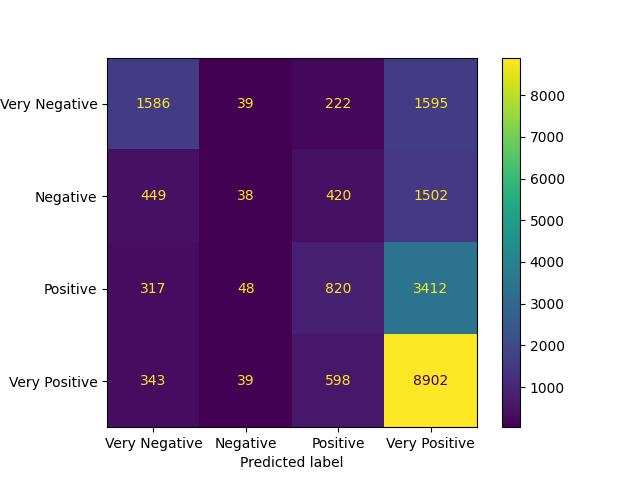
\includegraphics[width=0.7\linewidth]{conf_matrix_treeclf.png}
    \caption{Confusion matrix of the decision tree classifier.}
    \label{fig:decision_tree_conf}
\end{figure}

% Most important words
% Word: waste, Score: 0.006
% Word: worst, Score: 0.006
% Word: great, Score: 0.006
% Word: bad, Score: 0.005
% Word: want, Score: 0.005
% Word: love, Score: 0.005
% Word: movie, Score: 0.005
% Word: film, Score: 0.004
% Word: like, Score: 0.004
% Word: good, Score: 0.004


However, one advantage of decision trees is that they are interpretable. We can look at the most important words in the dataset that were used to make such decisions. When we look at these words, they are words that in many cases very clearly denote the sentiment of the review. For example, some of the most important words are "waste", "worst", "great", and "bad". These words are very clearly words that denote the sentiment of the review, and as a result the model is able to predict the sentiment of the review based on these words. As a result, we can confirm that despite not performing very well, the model is still able to learn some meaningful patterns in the data. The most important words can be seen in Table \ref{fig:decision_tree_words}.

% Table of the words 
\begin{table}
    \centering
    \begin{tabular}{|c|c|}
        \hline
        Word & Importance \\
        \hline
        waste & 0.006 \\
        worst & 0.006 \\
        great & 0.006 \\
        bad & 0.005 \\
        want & 0.005 \\
        love & 0.005 \\
        movie & 0.005 \\
        film & 0.004 \\
        like & 0.004 \\
        good & 0.004 \\
        \hline
    \end{tabular}
    \caption{Most important words in the decision tree classifier.}
    \label{fig:decision_tree_words}
\end{table}


\subsubsection{Deep Learning with DeBERTa}

Similarly, we train a deep learning model on the training set of the reviews. However, instead of TF-IDF vectors, we instead use the tokenizer of the model, since DeBERTa and other language models have a different, more optimized way, of representing words compared to a single vector like TF-IDF. We 

\printbibliography
\end{document}

% \title{CSSM Report}
% \author{shamdan17 }
% \date{January 2024}

% \begin{document}

% \maketitle

% \section{Introduction}

% \end{document}
